\documentclass{article}
\usepackage[round]{natbib}
\usepackage{amsmath,amssymb,amsfonts}%
\usepackage{geometry}%
\usepackage{color}
\usepackage{graphicx}
\usepackage{authblk}
\usepackage{nameref}
\usepackage[right]{lineno}
\usepackage{subcaption}
\usepackage{tikz}
\usetikzlibrary{calc,positioning}

\begin{document}

\linenumbers
\title{What is an Ancestral Recombination Graph?}
% First authors
\author{Author McAuthorface}
% Corresponding

\maketitle

% JK: this is a rough first pass for a slightly different paper. Needs
% substantial revision.
\begin{abstract}
It has recently become possible to infer genetic ancestry in the presence of
recombination at scale for the first time, enabling many
downstream applications in population and statistical genetics.
Such recombinant genetic ancestry is usually
referred to as an Ancestral Recombination Graph, or ARG.
% Note: slight repetition here with first sentence.
There are now multiple methods that can infer ARGs at a practical scale
and it is therefore vital that these methods can be systematically evaluated
and compared to determine their strengths and weaknesses.
Unfortunately, however, there is substantial confusion over
terminology and little agreement on shared standards for data interchange,
significantly hampering progress in this important area.
This confusion and lack of agreement on basic issues such as what does and
does not constitute an ARG is partly attributable to the historical
development of the term.
Originally rigorously defined as
a stochastic process (the coalescent with recombination) together with its
representation, an ARG is now understood to refer to any
concrete realisation of a recombinant genetic ancestry.
We show that the standard description of an ARG
in terms of common ancestor and recombination events
(inherited from the original stochastic process definition) is
ambiguous, fundamentally limited and an unsuitable basis for data interchange.
We provide a simple alternative definition of an ARG in which a node
corresponds to one of an individual's monoploid genomes, an edge
% jk-note: this is clumsy
defines a genetic ancestry relationship between two nodes,
and annotations on those edges define the precise patterns of
ancestry in intervals along the genome.
We use this framework to define some classifications and metrics of ARG nodes,
and discuss the properties of some recently developed inference methods.
% jk-note: this ends a bit flat - we should say other stuff like we clarify
% how the ARG relates the pedigree, etc, etc. Let's go through again when
% we have a reasonable draft.
\end{abstract}

\textbf{Keywords:} Ancestral Recombination Graphs

\section*{Introduction}
Inferring the genetic relationships between sampled genomes in the form of an
evolutionary tree is a necessary prerequisite for many analyses of species \citep{rannala2003genetics}, non (or
rarely) recombining sections of DNA \citep{cann1987mitochondrial,underhill2001annalsofhumangenetics} and viruses \citep{grenfell2004science}.
A genealogical tree captures what is known and
knowable about the genetic ancestry of the sample in an elegant and concise
way, by postulating a set of nodes that are ancestors common to the samples,
and the ancestral relationships between those nodes. A rich literature exists
on analysing the mathematical properties of these trees [cite?], and numerous
methods exist to infer them~\citep{felsenstein2004inferring}. The situation is
quite different in recombining organisms, where the analysis of genetic data
depends on summaries ultimately derived from the
trees~\citep{tajima1983evolutionary,tavare1984line}
such as allele frequencies and site frequency
spectra~\citep{achaz2009frequency,ralph2020efficiently},
patterns of linkage disequilibrium~\citep{mcvean2002genealogical}, and principal
components~\citep{mcvean2009genealogical}. Genealogical analysis is equally
fundamental to the study of recombining organisms, but profound technical
difficulties have made the routine inference of recombinant genealogies
impossible, and therefore tree-based analysis methods have been largely
unavailable to the fields of population and statistical
genetics.

Recent breakthroughs in large-scale inference
methods~\citep{rasmussen2014genome,kelleher2019inferring,speidel2019method,
schaefer2021ancestral,wohns2021unified}
and data representation~\citep{kelleher2016efficient}
have raised the genuine prospect of genealogical analysis becoming a standard part
of the population and statistical genetics toolkit~\citep{hejase2020summary}.
Applications using these inferred ancestries as input have
begun to appear~\citep{osmond2021estimating} and many more are sure to
follow~\citep{harris2019database}. This vibrant research area, however,
has a significant difficulty, which, if not addressed, will substantially hamper
progress. We currently lack a well-defined data-model and shared terminology
to discuss recombining genealogies,
leading to basic errors in statements about what different inference methods
produce as output (see the XXX section below), as well as presenting serious
difficulties in either comparing the outputs of different methods or
(from a users perspective) using multiple inference methods in an analysis.

In this paper we [turn into proper round up paragraph later]
\begin{enumerate}
\item Discuss the classical Ancestral Recombination Graph formulation,
and show how it derives from (and is limited by) the coalescent with
recombination.
\item Suggest a definition of ARGs that is free of these limitations,
where the formulation is derived from a (normally diploid) pedigree rather than from
coalescent approximations, and where the genetic
material which is transmitted is described by annotations attached to
edges rather than nodes.
\item Suggest a classification of ARG nodes that helps us to understand
the properties of the structures inferred by different methods, and illustrate
with some examples.
% Perhaps we should also mention something about simplification and unknowable
% nodes, e.g. "show how some of the nodes are not required for useful interpretation
% of ancestry".
\end{enumerate}

\section*{Ancestral graphs and stochastic processes}
The coalescent~\citep{kingman1982coalescent,kingman1982genealogy,
hudson1983testing, tajima1983evolutionary}
provides the theoretical underpinning for much of contemporary population genetics.
Hudson extended the coalescent to include
recombination~\citep{hudson1983properties,hudson1990gene}
and the model has proved to be an especially powerful basis for
simulations~\citep{hudson2002generating,baumdicker2021efficient}.
Hudson's algorithm is concerned with simulating the process of
the coalescent with recombination as efficiently as possible, and operates by
tracking segments of ancestral material carried by ancestors as
we go backwards in time. The details of Hudson's algorithm and how the
results of the ancestral process are represented are critical to later
discussions, and so we will explain the process in some detail.
See~\cite{kelleher2016efficient} for a more detailed
description of the algorithm, and how it may be implemented efficiently.


\begin{figure}[ht]
\centering
% FIXME this is a quick nasty hack to make the figure a bit smaller and
% prevent flushing all the other figures to the end of the document.
\scalebox{0.5}{
\begin{tabular}{cc}
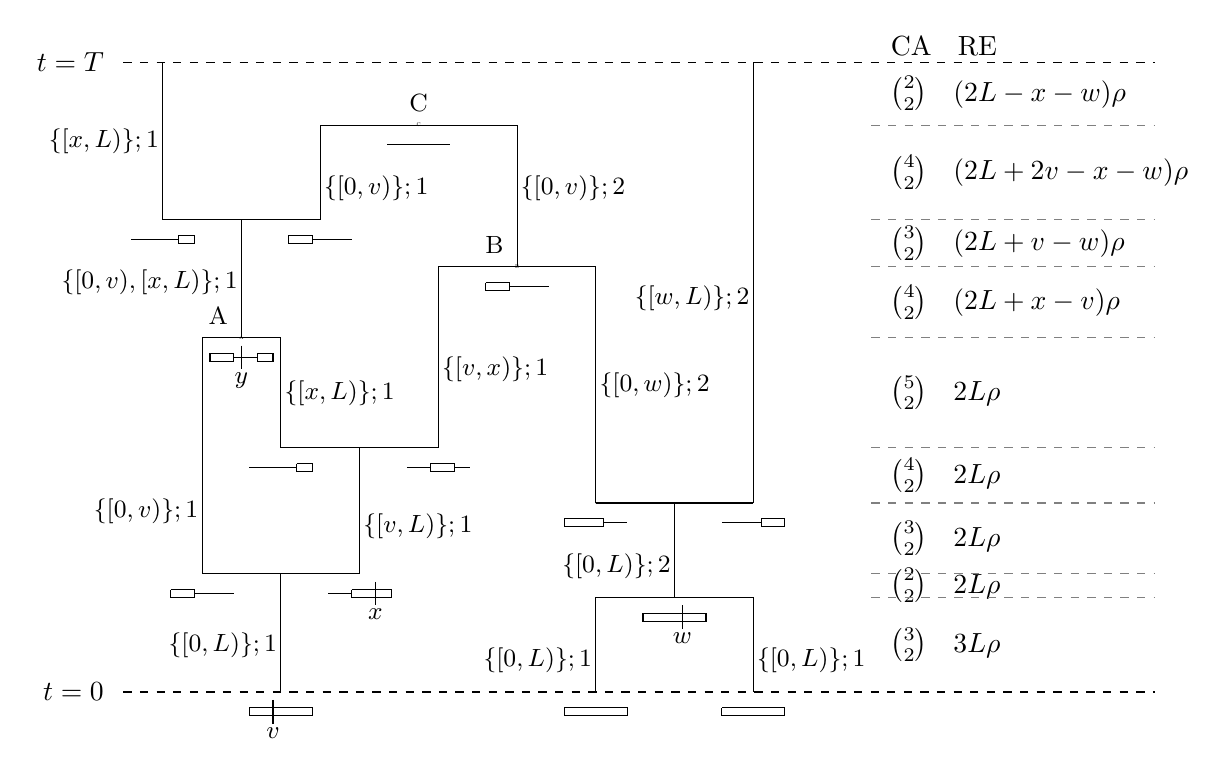
\begin{tikzpicture}
	\draw (-0.4, -0.2) -- (0.4, -0.2) -- (0.4, -0.3) -- (-0.4, -0.3) -- (-0.4, -0.2);
	\draw (-0.1, -0.1) -- (-0.1, -0.4);
	\node [label=below:{\small $v$}] at (-0.1, -0.2) {};
	\draw (3.6, -0.2) -- (4.4, -0.2) -- (4.4, -0.3) -- (3.6, -0.3) -- (3.6, -0.2);
	\draw (5.6, -0.2) -- (6.4, -0.2) -- (6.4, -0.3) -- (5.6, -0.3) -- (5.6, -0.2);

	\draw (4,0) -- (4, 1.2) -- (6, 1.2) -- (6,0);
	\draw (4.6, 1) -- (5.4, 1) -- (5.4, 0.9) -- (4.6, 0.9) -- (4.6, 1);
	\draw (5.1, 1.1) -- (5.1, 0.8);
	\node [label=below:{\small $w$}] at (5.1, 1) {};

	\draw (0, 0) -- (0, 1.5) -- (-1,1.5) -- (1,1.5);
	\draw (-1.4, 1.3) -- (-1.1, 1.3) -- (-1.1, 1.2) -- (-1.4, 1.2) -- (-1.4, 1.3);
	\draw (-1.1, 1.25) -- (-0.6, 1.25);
	\draw (0.6, 1.25) -- (0.9, 1.25);
	\draw (0.9, 1.3) -- (1.4, 1.3) -- (1.4, 1.2) -- (0.9, 1.2) -- (0.9, 1.3);
	\draw (1.2, 1.4) -- (1.2, 1.1);
	\node [label=below:{\small $x$}] at (1.2, 1.3) {};

	\draw (5, 1.2) -- (5, 2.4) -- (4,2.4) -- (6,2.4);
	\draw (3.6, 2.2) -- (4.1, 2.2) -- (4.1, 2.1) -- (3.6, 2.1) -- (3.6, 2.2);
	\draw (4.1, 2.15) -- (4.4, 2.15);
	\draw (5.6, 2.15) -- (6.1, 2.15);
	\draw (6.1, 2.2) -- (6.4, 2.2) -- (6.4, 2.1) -- (6.1, 2.1) -- (6.1, 2.2);

	\draw (1, 1.5) -- (1, 3.1) -- (0,3.1) -- (2,3.1);
	\draw (-0.4, 2.85) -- (0.2, 2.85);
	\draw (0.2, 2.9) -- (0.4, 2.9) -- (0.4, 2.8) -- (0.2, 2.8) -- (0.2, 2.9);
	\draw (1.6, 2.85) -- (1.9, 2.85);
	\draw (1.9, 2.9) -- (2.2, 2.9) -- (2.2, 2.8) -- (1.9, 2.8) -- (1.9, 2.9);
	\draw (2.2, 2.85) -- (2.4, 2.85);

	\draw (-1, 1.5) -- (-1, 4.5) -- (0,4.5) -- (0,3.1);
	\node [scale=0.2,label=above left:{\small A}] at (-0.5,4.5) {A};
	\draw (-0.9, 4.3) -- (-0.6, 4.3) -- (-0.6, 4.2) -- (-0.9, 4.2) -- (-0.9, 4.3);
	\draw (-0.6, 4.25) -- (-0.3, 4.25);
	\draw (-0.3, 4.3) -- (-0.1, 4.3) -- (-0.1, 4.2) -- (-0.3, 4.2) -- (-0.3, 4.3);
	\draw (-0.5, 4.4) -- (-0.5, 4.1);
	\node [label=below:{\small $y$}] at (-0.5, 4.3) {};

	\draw (4,2.4) -- (4,5.4) -- (2,5.4) -- (2,3.1);
	\node [scale=0.2,label=above left:{\small B}] at (3,5.4) {B};
	\draw (2.6, 5.2) -- (2.9, 5.2) -- (2.9, 5.1) -- (2.6, 5.1) -- (2.6, 5.2);
	\draw (2.9, 5.15) -- (3.4, 5.15);

	\draw (-0.5, 4.5) -- (-0.5, 6) -- (-1.5,6) -- (0.5,6);
	\draw (-1.9, 5.75) -- (-1.3, 5.75);
	\draw (-1.3, 5.8) -- (-1.1, 5.8) -- (-1.1, 5.7) -- (-1.3, 5.7) -- (-1.3, 5.8);
	\draw (0.1, 5.8) -- (0.4, 5.8) -- (0.4, 5.7) -- (0.1, 5.7) -- (0.1, 5.8);
	\draw (0.4, 5.75) -- (0.9, 5.75);

	\draw (0.5, 6) -- (0.5, 7.2) -- (3,7.2) -- (3,5.4);
	\node [scale=0.2,label=above:{\small C}] at (1.75,7.2) {C};
	\draw (1.35, 6.95) -- (2.15, 6.95);

	\draw (-1.5, 6) -- (-1.5, 8);
	\draw (6, 2.4) -- (6, 8);

	% Edge annotations above each event
	\node [label=left:{\small$\{[0,L)\};1$}] at (0.2,0.6) {};
	\node [label=left:{\small$\{[0,L)\};1$}] at (4.2,0.4) {};
	\node [label=right:{\small$\{[0,L)\};1$}] at (5.8,0.4) {};
	\node [label=left:{\small$\{[0,L)\};2$}] at (5.2,1.6) {};
	\node [label=left:{\small$\{[0,v)\};1$}] at (-0.8,2.3) {};
	\node [label=right:{\small$\{[v,L)\};1$}] at (0.8,2.1) {};
	\node [label=right:{\small$\{[0,w)\};2$}] at (3.8,3.9) {};
	\node [label=left:{\small$\{[w,L)\};2$}] at (6.2,5) {};
	\node [label=right:{\small$\{[x,L)\};1$}] at (-0.2,3.8) {};
	\node [label=right:{\small$\{[v,x)\};1$}] at (1.8,4.1) {};
	\node [label=left:{\small$\{[0,v), [x, L)\};1$}] at (-0.3,5.2) {};
	\node [label=right:{\small$\{[0,v)\};2$}] at (2.8,6.4) {};
	\node [label=left:{\small$\{[x,L)\};1$}] at (-1.3,7) {};
	\node [label=right:{\small$\{[0,v)\};1$}] at (0.3,6.4) {};

	% Dashed lines for start and end times
	\draw[dashed] (-2, 0) -- (11.1, 0);
	\node [label=left:{$t = 0$}] at (-2,0) {};
	\draw[dashed] (-2, 8) -- (11.1, 8);
	\node [label=left:{$t = T$}] at (-2,8) {};

	% Numbers of extant ancestors and links, from top to bottom
	\node[label=right:{CA \; RE}] at (7.5, 8.2) {};
	\node[label=right:{$\binom{2}{2}$ \; $(2 L - x - w) \rho$}] at (7.5, 7.6) {};
	\node[label=right:{$\binom{4}{2}$ \; $(2 L + 2 v - x - w) \rho$}] at (7.5, 6.6) {};
	\node[label=right:{$\binom{3}{2}$ \; $(2 L + v - w) \rho$}] at (7.5, 5.7) {};
	\node[label=right:{$\binom{4}{2}$ \; $(2 L + x - v) \rho$}] at (7.5, 4.95) {};
	\node[label=right:{$\binom{5}{2}$ \; $2 L \rho$}] at (7.5, 3.8) {};
	\node[label=right:{$\binom{4}{2}$ \; $2 L \rho$}] at (7.5, 2.75) {};
	\node[label=right:{$\binom{3}{2}$ \; $2 L \rho$}] at (7.5, 1.95) {};
	\node[label=right:{$\binom{2}{2}$ \; $2 L \rho$}] at (7.5, 1.35) {};
	\node[label=right:{$\binom{3}{2}$ \; $3 L \rho$}] at (7.5, 0.6) {};

	% Gray dashed lines to visually separate holding times
	\draw[color=gray, dashed] (7.5, 1.2) -- (11.1, 1.2);
	\draw[color=gray, dashed] (7.5, 1.5) -- (11.1, 1.5);
	\draw[color=gray, dashed] (7.5, 2.4) -- (11.1, 2.4);
	\draw[color=gray, dashed] (7.5, 3.1) -- (11.1, 3.1);
	\draw[color=gray, dashed] (7.5, 4.5) -- (11.1, 4.5);
	\draw[color=gray, dashed] (7.5, 5.4) -- (11.1, 5.4);
	\draw[color=gray, dashed] (7.5, 6) -- (11.1, 6);
	\draw[color=gray, dashed] (7.5, 7.2) -- (11.1, 7.2);
\end{tikzpicture}
&
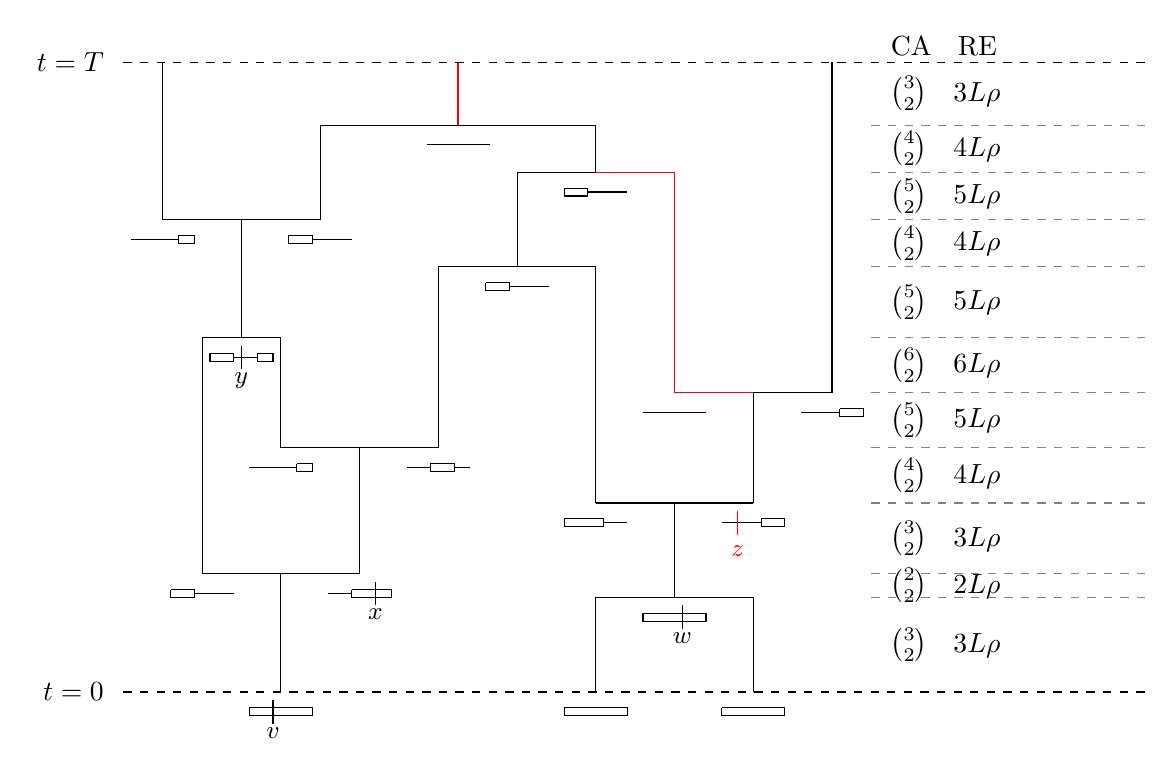
\begin{tikzpicture}
	\draw (-0.4, -0.2) -- (0.4, -0.2) -- (0.4, -0.3) -- (-0.4, -0.3) -- (-0.4, -0.2);
	\draw (-0.1, -0.1) -- (-0.1, -0.4);
	\node [label=below:{\small $v$}] at (-0.1, -0.2) {};
	\draw (3.6, -0.2) -- (4.4, -0.2) -- (4.4, -0.3) -- (3.6, -0.3) -- (3.6, -0.2);
	\draw (5.6, -0.2) -- (6.4, -0.2) -- (6.4, -0.3) -- (5.6, -0.3) -- (5.6, -0.2);

	\draw (4,0) -- (4, 1.2) -- (6, 1.2) -- (6,0);
	\draw (4.6, 1) -- (5.4, 1) -- (5.4, 0.9) -- (4.6, 0.9) -- (4.6, 1);
	\draw (5.1, 1.1) -- (5.1, 0.8);
	\node [label=below:{\small $w$}] at (5.1, 1) {};

	\draw (0, 0) -- (0, 1.5) -- (-1,1.5) -- (1,1.5);
	\draw (-1.4, 1.3) -- (-1.1, 1.3) -- (-1.1, 1.2) -- (-1.4, 1.2) -- (-1.4, 1.3);
	\draw (-1.1, 1.25) -- (-0.6, 1.25);
	\draw (0.6, 1.25) -- (0.9, 1.25);
	\draw (0.9, 1.3) -- (1.4, 1.3) -- (1.4, 1.2) -- (0.9, 1.2) -- (0.9, 1.3);
	\draw (1.2, 1.4) -- (1.2, 1.1);
	\node [label=below:{\small $x$}] at (1.2, 1.3) {};

	\draw (5, 1.2) -- (5, 2.4) -- (4,2.4) -- (6,2.4);
	\draw (3.6, 2.2) -- (4.1, 2.2) -- (4.1, 2.1) -- (3.6, 2.1) -- (3.6, 2.2);
	\draw (4.1, 2.15) -- (4.4, 2.15);
	\draw (5.6, 2.15) -- (6.1, 2.15);
	\draw (6.1, 2.2) -- (6.4, 2.2) -- (6.4, 2.1) -- (6.1, 2.1) -- (6.1, 2.2);
	\draw [color=red](5.8, 2.3) -- (5.8, 2.0);
	\node [label={[red]below:{\small $z$}}] at (5.8, 2.1) {};

	\draw (1, 1.5) -- (1, 3.1) -- (0,3.1) -- (2,3.1);
	\draw (-0.4, 2.85) -- (0.2, 2.85);
	\draw (0.2, 2.9) -- (0.4, 2.9) -- (0.4, 2.8) -- (0.2, 2.8) -- (0.2, 2.9);
	\draw (1.6, 2.85) -- (1.9, 2.85);
	\draw (1.9, 2.9) -- (2.2, 2.9) -- (2.2, 2.8) -- (1.9, 2.8) -- (1.9, 2.9);
	\draw (2.2, 2.85) -- (2.4, 2.85);

	\draw (-1, 1.5) -- (-1, 4.5) -- (0,4.5) -- (0,3.1);
	\draw (-0.9, 4.3) -- (-0.6, 4.3) -- (-0.6, 4.2) -- (-0.9, 4.2) -- (-0.9, 4.3);
	\draw (-0.6, 4.25) -- (-0.3, 4.25);
	\draw (-0.3, 4.3) -- (-0.1, 4.3) -- (-0.1, 4.2) -- (-0.3, 4.2) -- (-0.3, 4.3);
	\draw (-0.5, 4.4) -- (-0.5, 4.1);
	\node [label=below:{\small $y$}] at (-0.5, 4.3) {};

	\draw (6, 2.4) -- (6, 3.8) -- (7, 3.8);
	\draw [color=red](6, 3.8) -- (5, 3.8);
	\draw (4.6, 3.55) -- (5.4, 3.55);
	\draw (6.6, 3.55) -- (7.1, 3.55);
	\draw (7.1, 3.6) -- (7.4, 3.6) -- (7.4, 3.5) -- (7.1, 3.5) -- (7.1, 3.6);

	\draw (4,2.4) -- (4,5.4) -- (2,5.4) -- (2,3.1);
	\draw (2.6, 5.2) -- (2.9, 5.2) -- (2.9, 5.1) -- (2.6, 5.1) -- (2.6, 5.2);
	\draw (2.9, 5.15) -- (3.4, 5.15);

	\draw (-0.5, 4.5) -- (-0.5, 6) -- (-1.5,6) -- (0.5,6);
	\draw (-1.9, 5.75) -- (-1.3, 5.75);
	\draw (-1.3, 5.8) -- (-1.1, 5.8) -- (-1.1, 5.7) -- (-1.3, 5.7) -- (-1.3, 5.8);
	\draw (0.1, 5.8) -- (0.4, 5.8) -- (0.4, 5.7) -- (0.1, 5.7) -- (0.1, 5.8);
	\draw (0.4, 5.75) -- (0.9, 5.75);

	\draw [color=red](5, 3.8) -- (5, 6.6) -- (4, 6.6);
	\draw (4,6.6) -- (3,6.6) -- (3, 5.4);
	\draw (3.6, 6.4) -- (3.9, 6.4) -- (3.9, 6.3) -- (3.6, 6.3) -- (3.6, 6.4);
	\draw (3.9, 6.35) -- (4.4, 6.35);

	\draw (0.5, 6) -- (0.5, 7.2) -- (4,7.2) -- (4,6.6);
	\draw (1.85, 6.95) -- (2.65, 6.95);

	\draw (-1.5, 6) -- (-1.5, 8);
	\draw [color=red](2.25, 7.2) -- (2.25, 8);
	\draw (7, 3.8) -- (7, 8);

	% Dashed lines for start and end times
	\draw[dashed] (-2, 0) -- (11, 0);
	\node [label=left:{$t = 0$}] at (-2,0) {};
	\draw[dashed] (-2, 8) -- (11, 8);
	\node [label=left:{$t = T$}] at (-2,8) {};

	% Numbers of extant ancestors and links, from top to bottom
	\node[label=right:{CA \; RE}] at (7.5, 8.2) {};
	\node[label=right:{$\binom{3}{2}$ \; $3 L \rho$}] at (7.5, 7.6) {};
	\node[label=right:{$\binom{4}{2}$ \; $4 L \rho$}] at (7.5, 6.9) {};
	\node[label=right:{$\binom{5}{2}$ \; $5 L \rho$}] at (7.5, 6.3) {};
	\node[label=right:{$\binom{4}{2}$ \; $4 L \rho$}] at (7.5, 5.7) {};
	\node[label=right:{$\binom{5}{2}$ \; $5 L \rho$}] at (7.5, 4.95) {};
	\node[label=right:{$\binom{6}{2}$ \; $6 L \rho$}] at (7.5, 4.15) {};
	\node[label=right:{$\binom{5}{2}$ \; $5 L \rho$}] at (7.5, 3.45) {};
	\node[label=right:{$\binom{4}{2}$ \; $4 L \rho$}] at (7.5, 2.75) {};
	\node[label=right:{$\binom{3}{2}$ \; $3 L \rho$}] at (7.5, 1.95) {};
	\node[label=right:{$\binom{2}{2}$ \; $2 L \rho$}] at (7.5, 1.35) {};
	\node[label=right:{$\binom{3}{2}$ \; $3 L \rho$}] at (7.5, 0.6) {};

	% Gray dashed lines to visually separate holding times
	\draw[color=gray, dashed] (7.5, 1.2) -- (11, 1.2);
	\draw[color=gray, dashed] (7.5, 1.5) -- (11, 1.5);
	\draw[color=gray, dashed] (7.5, 2.4) -- (11, 2.4);
	\draw[color=gray, dashed] (7.5, 3.1) -- (11, 3.1);
	\draw[color=gray, dashed] (7.5, 3.8) -- (11, 3.8);
	\draw[color=gray, dashed] (7.5, 4.5) -- (11, 4.5);
	\draw[color=gray, dashed] (7.5, 5.4) -- (11, 5.4);
	\draw[color=gray, dashed] (7.5, 6) -- (11, 6);
	\draw[color=gray, dashed] (7.5, 6.6) -- (11, 6.6);
	\draw[color=gray, dashed] (7.5, 7.2) -- (11, 7.2);
\end{tikzpicture}
\end{tabular}
}
\caption{(A)
A realisation of the graph traversed by Hudson's algorithm started from a
sample of three continuous chromosomes of length $L$ at time $t = 0$, and
propagated until time $T$. The MRCA on the genetic interval $[v, w)$ is reached
at event B, while that on $[0, v)$ is reached at event C.
The non-ancestral segment $[v, w)$ above
A contributes to the rate of effective recombinations because it
is trapped between ancestral segments. The two columns titled CA and RE
are the respective rates of mergers and recombinations when
the recombination rate is $\rho$.
(B) A corresponding realisation of a big ARG, which augments Hudson's algorithm
by tracking nonancestral lineages. The result is a simpler state space and
dynamics, at the cost of extra nodes and edges, highlighted in red, which do
not affect the local tree at any site.}
\label{hudson_vs_bigARG}
\end{figure}

Hudson's algorithm operates by tracking the state of a set of ancestral
lineages as we go backwards in time.
% jk-note unclear here about the best choice of notation. We could have
% lists of tuples (l, r, a), or a tuple of vectors (l_j, r_j, a_j),
% of a tuple (I_j, a_j), where I is a vector of intervals. Going to
% stick with the original tuple notation for now.
%
% Each lineage consists of a set of
% equal-length vectors $\mathbf{l}$, $\mathbf{r}$ and $\mathbf{a}$
% such that for each $1 \leq j \leq \left| l \right|$,
% $[\mathbf{l}_j, \mathbf{r}_j)$ is a half-closed genomic interval and
% $\mathbf{a}_j$ is an integer
% tracking the number of samples the lineage is ancestral to over the interval.
% Assume that the intervals are sorted from left-to-right so that $\mathbf{l}_1$
% and $\mathbf{r}_{|\mathbf{r}|}$ are the left- and right-most positions
% covered by the lineage, respectively.
Each lineage consists of a list of
disjoint ancestry segments $(\ell, r, a)$, where
$[\ell, r)$ is a half-closed genomic interval and $a$ is an integer
tracking the number of samples to which the lineage is ancestral over that interval.
(We also usually track the tree node associated with each segment, but
that is not important for our purposes here so we omit it.)
If we have $n$ samples and a genome of length $m$, the process begins with $n$ lineages
of the form $\{(0, m, 1)\}$. The process then works backwards in time from
the present day as a series of random common ancestor or recombination events.
Recombination events occur at a rate determined by the amount of ancestral material and
the way in which it is distributed along a chromosome.
Let $L$ be the set of ancestors at a given time $t$. Recombination events
happen at rate $\rho \nu / (m - 1)$ where
\[
\nu = \sum_{x \in L}\left( \max_{(\ell, r, a) \in x}r
    - \min_{(\ell, r, a) \in x}\ell - 1 \right)
\]
is the number of available `links' that may be broken. Thus, the rate of
recombination is determined by the left- and right-most extent of the
ancestral material carried by each lineage. At a recombination
event we choose one of these links uniformly and break it. Given a lineage
$x = [(\ell_j, r_j, a_j)]$ and a breakpoint $k$, we have two lineages
$x_1$ and $x_2$ such that FILL IN DETAILS

When $k = |L|$ lineages are present, common ancestor events
occur at rate $\binom{k}{2}$. In a common ancestor event, two lineages
are chosen uniformly at random and their ancestry segments merged.
If we have overlapping intervals of ancestry from the two lineages,
say, $(\ell, r, a_1)$ and $(\ell, r, a_2)$, a
\emph{coalescence} occurs and ancestor represented by the current event
will be present as a node (at least) in the marginal trees covering
the interval $[\ell, r)$. The result of this coalescence is a segment
$(\ell, r, a_1 + a_2)$, and if $a_1 + a_2 < n$ it is included in the
ancestry for the new lineage. Otherwise, if $a_1 + a_2 = n$ we know that
we have found the most recent common ancestor of all samples in
the interval $[\ell, r)$ and so we do not need to simulate its history any further.
Nonoverlapping intervals of ancestry from the two lineages are included
in the resulting lineage without changes. Eventually, as the process continues,
we find resultant lineages in which all segments have fully coalescenced,
and so the number of extant lineages gradually dwindles down to zero.

% NOTE: it would probably be helpful to have a drawing of the ARG process
% in-progress here to help us talk about it. What is the full state
% that is remembered as we go through the process? It does help to think
% about the process as choosing edges to merge, not nodes.
The Ancestral Recombination Graph (ARG) was later introduced by
Griffiths~\citep{griffiths1991two,ethier1990two,griffiths1996ancestral,
griffiths1997ancestral}, and is a
closely related and complementary treatment of the same process. Where
Hudson's algorithm is focused on the efficient \emph{simulation} of the
process, the original ARG literature is focused on mathematical
results about the stochastic process. Griffiths and colleagues used the word
``ARG'' to refer to both a specific branching-coalescing stochastic process and
the graph structure derived from this process. For clarity, we will refer to the
process as the Griffiths process, or the coalescent with recombination (CwR),
and following XX-Who?-XX, we refer to the the structure as the ``big ARG'', as
opposed to the ``little ARG'' traversed by Hudson's algorithm
(\citet{wiuf1999recombination} refer to these structures as ARG and HUD respectively).

In the Griffiths formulation, each edge in the graph corresponds to an extant
lineage and nodes are events in the process (the initial $n$ leaf nodes are
``sampling'' events). As in Hudson's
algorithm, common ancestor events occur at rate $\binom{k}{2}$ when there
are $k$ lineages present. We choose two lineages (edges) uniformly, and merge them
into a common ancestor lineage. Recombination events are different
to Hudson's algorithm, however. Rather than occuring at a rate which depends on
the specific distribution of ancestral material among lineages, the
rate of recombination is now simply $k \rho (m - 1)$. At a recombination event
we choose a lineage (edge) uniformly, and a
breakpoint $0 < x < L$ uniformly on its genome. We terminate the edge at a
node, record the breakpoint and start two new edges from this node. The process
then continues until there is only one lineage left (the Grand Most Recent
Common Ancestor, GMRCA), which is guaranteed to
happen in finite time because of the linear vs quadratic rates of branching
and coalescing. The graph structure and breakpoints associated with
recombination nodes provides sufficient information to later recover the marginal
trees (see the next section for more details and discussion on this point).

The state-space of the Griffiths process is much simpler than Hudson's algorithm,
which greatly facilitates mathematical reasoning. This simplicity comes at a
substantial cost, however, if we wish to use it as a practical means of
simulating recombinant ancestry. The big ARG is vast, and any realisation
for even moderate levels of recombination is far too large to be of practical
use. The number of events in the big ARG, all the way back to the GMRCA
is $O(e^\rho)$~\citep{griffiths1997ancestral}, whereas the number
of events required to simulate the little ARG is
$O(\rho^2)$~\citep{hein2004gene,baumdicker2021efficient}.
This disparity in the number of events in the two formulations is
because the majority of the events that occur in the big ARG do
not affect the genetic ancestry of the sample in any way. Recombination
events that occur outside of ancestral material do not have any bearing
on the ancestry of the sample, and so the structure is hugely redundant.
As~\cite{wiuf1999recombination} note,
``an `ancestral' sequence in the birth and death process
need not have any genetic material in common with a
sequence descended from it.''

% Full quote:
% This process simplifies mathematics on the account that the notion of an
% ancestor will have a less restrictive meaning than usual:
% An ``ancestral'' sequence in the birth and death process
% need not have any genetic material in common with a
% sequence descended from it.

[Review of other work done on the ARG stochastic process here.
Discuss \citet{wiuf1999ancestry}. Wiuf and Hein's classical pair of papers
clarified the relationship between Hudson's algorithm and the ARG.
Explain that ARG simulation is inherently less efficient than Hudson's
algorithm because we must track all lineages, even those that correspond
to sections that have coalesced, or we won't have a complete ARG.
This might be tricky to communicated without a figure, but is an
esoteric point perhaps not worth spending a figure on.]

Similar graph encodings have also been introduced to model other mechanisms
which change the local ancestral tree along the genome, such as gene
conversion~\citep{wiuf2000coalescent} and
horizontal gene transfer~\citep{baumdicker2014infinitely}.
[Mention the
SMC~\citep{mcvean2005approximating,marjoram2006fast}
and ClonalFrame~\citep{didelot2007inference} approximations somewhere.]

The idea of using branching-coalescing stochastic processes
to model genetic ancestral trees has also found application in natural selection.
The Ancestral Selection Graph (ASG)~\citep{krone1997ancestral,neuhauser1997genealogy}
uses dynamics identical to the ``big'' ARG to simulate an ensemble of correlated
potential ancestral trees. Weak genic selection is incorporated by sampling a
true ancestry from the ensemble in a non-uniform way.
There is no ASG analogue of the more computationally tractable ``little'' ARG,
though some gains in tractability can be made by considering typed
lineages~\citep{etheridge2009coalescent} or by leveraging perfect simulation
techniques when recurrent mutation is present\citep{fearnhead2001perfect}.
Extensions of the ASG have been developed to frequency-dependent
selection~\citep{neuhauser1999ancestral, gonzalezcasanova2018duality},
unlinked chromosomes~\citep{fearnhead2003ancestral}, recombining
loci whereupon branching is due to both selection and
recombination~\citep{donnelly1999genealogical}, and high fecundity
reproduction~\citep{gonzalezcasanova2018duality, koskela2019robust}.

\section*{The Event ARG data structure}
% When did we move from the ARG is a process to the ARG is a data structure?
% What was the historical progression from one to the other?
Early work on ARG inference focused on the problem of
of inferring parameters of the
stochastic process, where the ancestry is regarded as a
latent parameter to be averaged out
\citep[e.g.][]{griffiths1996ancestral,kuhner2000maximum, nielsen2000estimation,
fearnhead2001estimating}. These methods met with limited success
due to the overwhelmingly large and
horribly structured [Jere: what's the right way to say this?]
state space of ARGs. The focus subsequently shifted to
the more tractable---but still
NP-hard~\citep{wang2001perfect}---problem of computing
the minimum number of recombinations required
to explain an input dataset [CITATIONS], and inferring the corresponding
ARG realisations~\citep{song2003parsimonious,song2005efficient,lyngso2005minimum}.
The distinction between the ARG as a stochastic process
and the ARG as a data structure became less clear at this point,
with \citet{minichiello2006mapping} explicitly arguing for
the data structure interpretation.

% What do we mean by an EARG, informally?
The Griffiths ARG encoding is an elegant and mathematically
economical description of the coalescent with recombination on a single
chromosome, but it has significant drawbacks as the basis for a general purpose
storage and interchange format. To avoid confusion, we will refer to this
ARG encoding as an ``Event ARG'', or EARG.
The basic unit of an EARG are \emph{events} and correspond directly
to the events that
occur in the ARG stochastic process described in the previous section.
Each event corresponds to a node in the graph, and there are therefore
two types of node: common ancestor and recombination. As in the
stochastic process, edges represent lineages, and those lineages
are modified by the events that they pass through.

% What do we mean by an EARG, formally?
% NOTE we're using the natural numbers but are using 0 as a node in the
% examples. Probably want to clear this up a bit.
Formally, we can define an EARG as a tuple $(e, \sigma)$, where $e$
defines a directed acyclic graph where $e_j = (c, p)$ describes
an edge between
child node $c$ and parent $p$ ($c, p \in \mathbb{N}$).
Additionally,
$\sigma: \mathbb{N} \rightarrow \mathbb{N}$
is a function mapping nodes to recombination breakpoints, such that $\sigma(u) = x$
if $u$ is a recombination event with breakpoint $x$ and
$\sigma(u) = \infty$ otherwise. (The use of $\infty$ to denote
non-recombination nodes is arbitrary, but useful when we extract
% NOTE: need to be careful about using "local" trees if we're also
% distinguishing resolved and non-resolved GARGs as being "locally"
% defined or not. One is topologically local and the other is local
% along the genome.
local trees; see below.)
For each recombination node $u$ we must
have exactly two edges in $E$ such that $u$ is the child.
Note that this description captures only the
graph topology: if we also wish to know the times of events we need
an additional function $t(u): \mathbb{N} \rightarrow \mathbb{R}$
which defines the time of each node.
An example is given in Fig.~\ref{fig-arg-data-structure}A.

\begin{figure}
\centering
\begin{tabular}{cc}
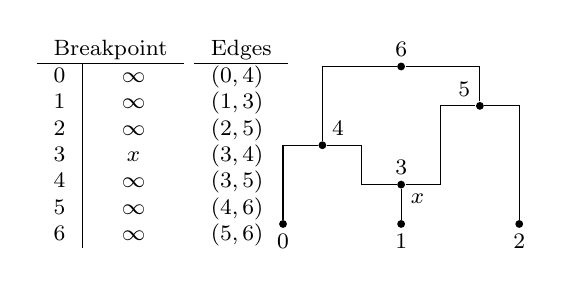
\begin{tikzpicture}[x=5mm, y=5mm, node distance=2mm and 20mm]
\tikzset{greynode/.style={circle,fill,inner sep=1},
nodelabel/.style={font=\footnotesize}}

\node (s0) [greynode] at (0, 0) {};
\node (s1) [greynode] at (3, 0) {};
\node (s2) [greynode] at (6, 0) {};
\node (s3) [greynode] at (3, 1) {};
\node (s4) [greynode] at (1, 2) {};
\node (s5) [greynode] at (5, 3) {};
\node (s6) [greynode] at (3, 4) {};

\node [nodelabel,anchor=north west] at ($(s3) + (0,0)$) {$x$};
\foreach \u/\lab in {s0/0, s1/1, s2/2} \node[nodelabel,anchor=north] at (\u) {\lab};
\foreach \u/\lab in {s4/4} \node[nodelabel,anchor=south west] at (\u) {\lab};
\foreach \u/\lab in {s5/5} \node[nodelabel,anchor=south east] at (\u) {\lab};
\foreach \u/\lab in {s3/3, s6/6} \node[nodelabel,anchor=south] at (\u) {\lab};

%% Edges
\draw (s1) -- (s3);
\draw (s0) |- (s4);
\draw (s4) -- (2,2) |- (s3);
\draw (s4) |- (s6);
\draw (s3) -- (4,1) |- (s5);
\draw (s2) |- (s5);
\draw (s5) |- (s6);

\node [nodelabel,anchor=north west] at ($(-6.5,5)$) {
\begin{tabular}{c|c}
\multicolumn{2}{c}{Breakpoint}\\
\hline
0 & $\infty$ \\
1 & $\infty$ \\
2 & $\infty$ \\
3 & $x$ \\
4 & $\infty$ \\
5 & $\infty$ \\
6 & $\infty$ \\
\end{tabular}};

\node [nodelabel,anchor=north west] at ($(-2.5,5)$) {
\begin{tabular}{l}
Edges\\
\hline
$(0, 4)$ \\
$(1, 3)$ \\
$(2, 5)$ \\
$(3, 4)$ \\
$(3, 5)$ \\
$(4, 6)$ \\
$(5, 6)$ \\
\end{tabular}};

\end{tikzpicture}
&
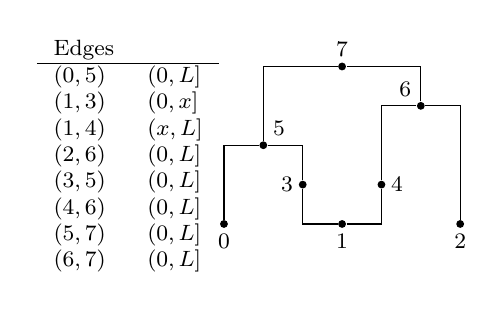
\begin{tikzpicture}[x=5mm,y=5mm,node distance=2mm and 20mm]
\tikzset{greynode/.style={circle,fill,inner sep=1},
nodelabel/.style={font=\footnotesize}}

\node (s0) [greynode] at (0, 0) {};
\node (s1) [greynode] at (3, 0) {};
\node (s2) [greynode] at (6, 0) {};
\node (s3) [greynode] at (2, 1) {};
\node (s4) [greynode] at (4, 1) {};
\node (s5) [greynode] at (1, 2) {};
\node (s6) [greynode] at (5, 3) {};
\node (s7) [greynode] at (3, 4) {};

\foreach \u/\lab in {s0/0, s1/1, s2/2} \node[nodelabel,anchor=north] at (\u) {\lab};
\foreach \u/\lab in {s3/3} \node[nodelabel,anchor=east] at (\u) {\lab};
\foreach \u/\lab in {s4/4} \node[nodelabel,anchor=west] at (\u) {\lab};
\foreach \u/\lab in {s5/5} \node[nodelabel,anchor=south west] at (\u) {\lab};
\foreach \u/\lab in {s6/6} \node[nodelabel,anchor=south east] at (\u) {\lab};
\foreach \u/\lab in {s7/7} \node[nodelabel,anchor=south] at (\u) {\lab};

%% Edges
\draw (s1) -| (s3);
\draw (s1) -| (s4) |- (s6);
\draw (s3) |- (s5);
\draw (s0) |- (s5);
\draw (s2) |- (s6);
\draw (s5) |- (s7);
\draw (s6) |- (s7);

\node [nodelabel,anchor=north west] at ($(-5,5)$) {
\begin{tabular}{ll}
Edges\\
\hline
$(0, 5)$ & $(0, L]$ \\
$(1, 3)$ & $(0, x]$ \\
$(1, 4)$ & $(x, L]$ \\
$(2, 6)$ & $(0, L]$ \\
$(3, 5)$ & $(0, L]$ \\
$(4, 6)$ & $(0, L]$ \\
$(5, 7)$ & $(0, L]$ \\
$(6, 7)$ & $(0, L]$ \\
\end{tabular}};

\end{tikzpicture}
\\
(A) & (B) \\
\end{tabular}
\caption{\label{fig-arg-data-structure}
Encoding an ARG. (A) The classical approach described by Griffiths
equates graph nodes with events in the stochastic process,
and associates recombination breakpoints with nodes. This encoding
is limited in the ancestral patterns that can be described and ambiguous.
[TODO clarify that the function is the same things as having two
types of nodes]
(B) Equating graph nodes with \emph{genomes} and attaching the
interval of genome inherited by the child node with edges removes
this ambiguity and can describe any pattern of genetic inheritance.
The most important change between the two encodings is to represent
a recombination event (node 3 in A) by two parent genomes
(nodes 3 and 4 in B) and explicitly storing the interval
that the child inherits from each parent along the two corresponding
edges. Thus, child $1$ in inherits $(0, x]$ from $3$
and $(x, L)$ from $4$
(for recombination breakpoint $x$ and a sequence of length $L$).
\textcolor{red}{This is very much a draft; let's see how it works with
 the text and other figures and tidy it up in a later revision}
}
\end{figure}

% % Not sure if we actually include this, but it's good to work it through
% % to make sure the notation works. Maybe something to stick into
% % an appendix
% The most fundamental operation that we need to perform on an ARG
% data structure is extracting the local tree topology at a particular
% position along the genome. The basic strategy is to traverse
% the graph upwards, building the tree as we visit each node.
% At a recombination node, when we have a choice of two parents,
% we follow the path that corresponds to the position that we
% are building the tree for. More precisely, let $S$ be the set
% of sample nodes (usually the leaves of the graph)
% and $0 \leq x < L$ be a position along the genome, and suppose
% we are building a mapping $p_u$ that defines the parent of node
% $u$ at $x$.
% Let $N$ be a set of
% nodes we are currently constructing the tree at,
% and initialise $N \leftarrow S$.
% Then, while $|N| > 0$, we add branches to the
% tree as follows. Let $u$ be an arbitrary element of $N$ (which
% we remove).
% % This isn't right: we're not handling the case where there's
% % no edges in E where the child is $u$.
% Then, if $\sigma(u) < x$ we let $j$ be the
% smallest value such that $e_{j,1} = u$, and otherwise
% let $j$ be the largest value such that $e_{j,1} = u$.
% Then, set $v \leftarrow e_{j, 2}$,
% $p_u \leftarrow v$
% and $N \leftarrow N \cup \{v\}$.

The ordering of edges is a vital element of the EARG encoding.
This is because there is a fundamental ambiguity involved
in associating recombination breakpoints with \emph{nodes}
rather than edges,
and the only way we can break this symmetry is to assign
some meaning to the order in which the parents are listed
(\cite{griffiths1997ancestral} refer to the ``left'' and ``right''
parents of a recombination event). When we want to recover
the local tree at a position $x$ along the genome,
we traverse the graph upwards from the leaves. At a particular
node $u$, if it has one parent we are at a common ancestor
node and we simply follow that parent. If we are at a
recombination node, $u$ has two parents; if
$x$ is less than the breakpoint $\sigma(u)$ we follow
the first edge, and otherwise follow the second edge.
This ordering requirement, which although straightforward
to describe, has some drawbacks in practice. For example,
% Surely the meaning is clear from the context here and we don't need
% qualify the meaning of "ARG"
simulating an ARG in this representation is
complicated by the fact that the
first event to occur may hit the lineage carrying the ancestry
to the right of the breakpoint rather
than the left (and so we cannot emit edges as they are generated).
Such issues can be worked around, of course,
but depending on the ordering of otherwise indistinguishable
objects is generally problematic. In practice, several
methods
explicitly associate information with the outbound edges
of a recombination event
to resolve the problem~\citep{lyngso2005minimum,ignatieva2021kwarg}.

% it's not reasonable to assume that one type of event happens
% at a time any more.
The Griffiths ARG encoding is also limited in the types of ancestral
history that can be described. This ARG encoding is derived from the coalescent
with recombination, which explicitly assumes that only one type
of event can occur (i.e., common ancestry or recombination) at a
time. This model is derived as an approximation to a Wright-Fisher
model, assuming that the sample size $n$ is much less than the
population size $N$ and [some assumptions about genome length]
\textcolor{red}{what is this Jere?}. While these approximations are
reasonable
to make when studying the Kreitman \emph{Drosphila Melanogaster}
dataset~\citep{kreitman1983nucleotide} ($n=11$, $N\approx 10^6$,
at 43 variant sites over x Kb \textcolor{red}{details and citation
for Ne estimate}) that is classically used for benchmarking
ARG inference methods [cites],
they are highly questionable in modern datasets. % absurd really
For example, there are now many
human datasets consisting of hundreds of thousands of
genomes~\citep{bycroft2018genome,karczewski2020mutational,tanjo2021practical},
and thus our sample size is often much \emph{larger} than $N_e$
(often assumed to be $10^4$ in humans).
% TODO make this better. Ask Gregor for some refs?
% Basically, Ag datasets make the assumption of isolated
% rare recombinations absurd.
Agricultural datasets such as the 1000 bull genomes~\citep{hayes20191000}
combine genome sequence data with detailed pedigrees, with
sample data from multiple generations.
Complete chromosome-level assemblies are now possible
in humans~\citep{miga2020telomere},
and projects are under way to obtain high-quality assemblies
for all eukaryotic species in Britain and Ireland~\citep{darwin2022sequence}
and ultimately worldwide~\citep{lewin2022earth}.
While the coalescent model can be suprisingly robust to such
basic violations to the underlying assumptions~\citep{
wakeley2012gene,bhaskar2014distortion,nelson2020accounting},
it is not acceptable that our ability to \emph{represent}
ancestral relationships should be limited by these assumptions.
In a Wright-Fisher model, coalescence and recombination can
occur at the same time in the same genomes, and we can be
certain that this is also true in the incredibly rich
datasets that are available today.

Another limitation of the Griffiths ARG encoding illustated in
Fig.~\ref{fig-arg-data-structure}A is the inability to represent
multiple recombinations along a chromosome, gene conversion,
or transmission of multiple chromosomes.
[Sentence saying ``gene conversion is important, actually, cite, cite,
so we should be hoping to infer it some day''. Presumably people
already are in bacterial contexts?]
To allow us to encode data from these important processes we
must either devise workarounds to the event based encoding
(i.e., model gene conversion as two recombination events) or
generalise the model to more appropriately reflect the realities
of modern datasets.

Fortunately, it is straightforward to generalise the classical Griffiths
encoding to both simplify implementations and to encompass any
possible pattern of genetic inheritance.
We require only two changes. Firstly, we let nodes in the
graph model \emph{genomes} rather than \emph{events}. As we
see in the next section, this allows us to model complex
patterns of inheritance without classifying different types of node.
The second change we must make is to associate
the details of inheritance intervals with \emph{edges} rather than
as breakpoints associated with recombination events and
edge ordering rules.
% That is, given two genomes $p$
% and $c$ where $p$ is the parent genome and $c$ is the child
% (although many generations may have elapsed between the two),
% we associate a set $I$ of intervals of genome which $c$ has
% inherited from $p$.
These changes are straightforward, involve no loss of information
and greatly increase both the expressivity and computational
power of ancestral recombination graph data structures.

\section*{Genome ARGs}
% We're not the first to talk about ARGs and pedigrees, and we're
% not doing anything controversial.
The deep connection between ARGs and pedigrees is of course
well known
\citep[e.g.][]{wakeley2012genetics,gusfield2014recombinatorics,
speed2015naturereviewsgenetics}
and recent discussions have illustrated the
relationship~\citep{mathieson2020ancestry,brandt2021evaluation}, % more??
showing how the coalescence and recombination events in an ARG
correspond to particular genomes in the pedigree.
As discussed in the previous section, the definition of an ARG
as a \emph{data structure} in terms of these two events is problematic,
fundamentally limiting the patterns of ancestry that can be described.
Following \cite{mathieson2020ancestry} we instead define the
ARG data structure \emph{in terms of} an underlying pedigree, so that
any form of inheritance structure can be modelled.
% Bit of duplication here, but good to make the point about being
% motivated by real existing datasets not some academic desire to
% model complexity that isn't there.
This, coupled with
the explicit association of genome coordinates with edges, allows
us to represent even the bewilderingly complex patterns of relatedness
present in modern datasets.

\begin{figure}
\begin{center}
    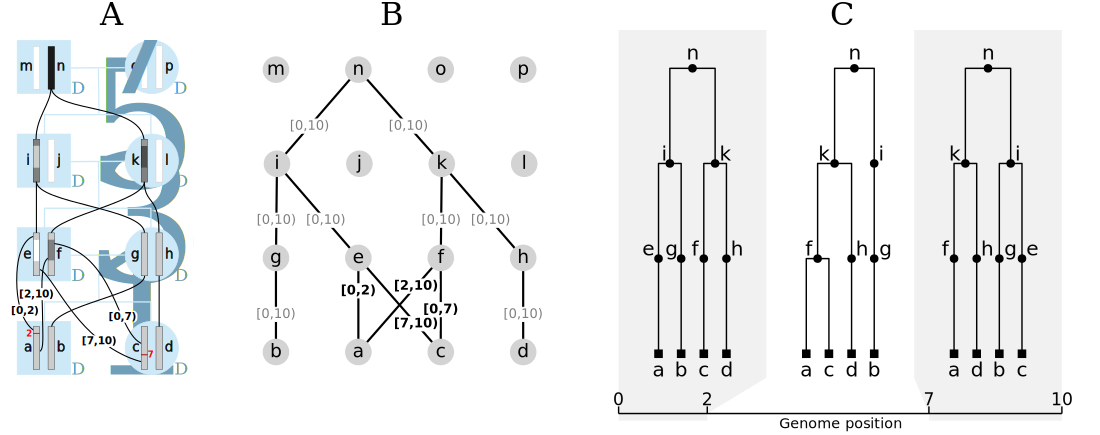
\includegraphics[width=\textwidth]{illustrations/arg-in-pedigree}
\end{center}
\caption{\label{fig-arg-in-pedigree}
% TODO caption needs another pass. One the full section has been written
% it'll be clearer what we need to say in the caption vs the text.
The Ancestral Recombination Graph defined as arbitrary inheritance
of genomes between diploid (or any ploidy; see text) individuals.
(A) Each individual consists of two genomes, and each genome is
inherited as a (potentially) recombinant mixture of the individual's parent's
genomes. (B) Genomes are modelled as nodes in a graph, and the edges
denote inheritance. Each edge is annotated with genome coordinates
defining the specific region(s) inherited.
(C) This description of inheritance fully defines the
local relationships along the genome, as shown in the local
or ``marginal'' trees.
}
\end{figure}

To distinguish from the classical event-based encodings,
we call this encoding of an ARG data
structure a ``Genome ARG'', or GARG.
Fig~\ref{fig-arg-in-pedigree} illustrates the basic elements of a GARG.
The pedigree is composed of a set of individuals who each carry
two \emph{genomes} (we assume diploidy here for concreteness, but there
is no inherent limitation on ploidy).
Each genome is inherited from one of the individual's parents, and may
be the recombined product of that parent's two genomes.
For example, individual $I_1$ in Fig.~\ref{fig-arg-in-pedigree}A
has two genomes $A$ and $B$,
inherited from parents $I_3$ and $I_4$. Genome $A$ is the product of
recombining $I_3$'s two genomes $E$ and $F$ at position FIXME,
whereas $B$ was inherited directly from $I_4$'s genome $G$ without
recombination. The pedigree is shown here for concreteness, but
is not a necessary part of the model. We can reason directly about the
genomes without necessarily knowing how they are combined within
individuals. This ``genome-perspective'' is show in
Fig.~\ref{fig-arg-in-pedigree}B, which depicts the same graph
of the ancestry of the sample genomes $A$--$D$. The graph
topology along with the genome coordinate annotations on the
edges then uniquely defines the trees at every position
along the genome (Fig.~\ref{fig-arg-in-pedigree}C).

The focus on modelling genomes rather than events has some interesting
and important consequences. Firstly, the graph may contain nodes that
do not correspond to any particular event in the ancestry of the
samples. For example, node $H$ is the direct ancestor of $D$ in
Fig~\ref{fig-arg-in-pedigree}, and is not the product of either a
coalescence or a recombination. Such nodes would usually be removed
from the graph so that $D$ descends directly from $K$ (see section XXX)
but there is no necessity for this from a representational perspective.
This ability can be useful in practice and could be required if,
% Do we need to spell this out?
for example, we have a deeply sequenced pedigree of
haplodiploids. % e.g. Honeybees? Be great to cite an example!

Secondly, the way that we model recombination is subtly different.
Rather than having a single node that represents the \emph{event},
there are three nodes (representing the recombinant offspring and
two parental genomes) and two edges with associated genome coordinate
intervals (representing the precise inheritance patterns).
For example, in Fig~\ref{fig-arg-in-pedigree}, node $A$ is the
recombinant descendent of $E$ and $F$, inheriting positions
FIXME from $E$ and genome positions FIXME from $F$. Any particular
node can be both a recombinant (it is the recombined product of
its parent's genomes) and a common ancestor (the ancestry from
multiple samples meet at this node; see the next section).
[More stuff here: clarify why we assign coordinates to edges
rather than nodes. Basically lay out all the stuff that we can
talk about \emph{without} going in to the details of
ancestry resolution.]


Formally, we can define a GARG as a set of edges $E$, where each
element of the set is a tuple $(c, p, I)$ such that $c, p \in \mathbb{N}$,
$c$ is the child node, $p$ is the parent node and $I$ is the set of
disjoint genomic intervals $(\ell, r]$ over which genome $c$ inherits from $p$ (we may
also phrase this in terms of the ancestral material of a sample---see
the next section). Deriving the local tree at a point $x$
follows largely the same pattern as for an EARG but is somewhat
simpler because coordinate information is directly associated with
edges. Starting with the sample nodes $S$ we traverse
upwards through the graph from child to parent. At each node $u$, we find an
edge $(c, p, I) \in E$ such that $u = c$ and $x \in I$ (if it
exists) and move to the next node $p$.

% Asking the reader to flick back to figure 2 here, not great.
The differences between EARGs
and GARGs are subtle but important, and illustrated in
Fig.~\ref{fig-arg-data-structure}, which shows a simple ARG
with three samples and one recombination.
Fig.~\ref{fig-arg-data-structure}A shows this topology as a
classical Griffiths-like EARG, and
Fig.~\ref{fig-arg-data-structure}B shows it as a GARG.
The two are almost identical, except we model the recombination
event via the two parental genomes in nodes $3$ and $4$ and explicitly
store the genomic interval that the child inherited from the
parent with every edge.
This approach may seem wasteful since we must store an extra
node for each recombination and genomic interval information
with every edge (even though many simply span the full genome).
However, asymptotically the amount of information stored is the
same, and as we see in the next section, keeping interval
information for all edges enables useful generalisations.
There is also much simplicity to be gained by having
a single type of node and by treating all edges in the same way.

\textcolor{red}{TODO: reduce this down to one paragraph, which
defines the relationship between what we define as an ARG and
what people mean by phylogenetic networks from the literature.
We probably don't need to get into quite so much detail on
the different types that people have studies. Essentially,
we're ending the section with a brief review which situates
our definition in the literature. I think pulling apart the
idea of a ``reticulation'' vs what we call a recombinant
is essential here.}

The term \emph{phylogenetic network} has been broadly accepted to describe the most general
type of genealogical graph, defined by \citet{huson2010phylogenetic} as ``any graph used to
represent evolutionary relationships (either abstractly or explicitly) between a set of taxa
that labels some of its nodes'' (although more narrow and context-dependent definitions can also
be found in the literature). Explicit rooted phylogenetic networks are rooted DAGs,
with leaves labelled by the taxa (species, groups, individuals or sequences), and nodes classed
as either reticulation nodes (with in-degree $\geq 2$) or tree nodes.

Some sub-classes of explicit rooted phylogenetic networks are defined based on the evolutionary event that the
reticulation nodes capture \citep{huson2010phylogenetic}. In \emph{reassortment} networks, used to
model the evolution of viruses, reticulation nodes correspond to exchange of
(non-recombining) genomic segments between viral particles inside a co-infected host.
In \emph{hybridisation} networks, reticulation nodes correspond to genetic material from two
different species combining to create a hybrid. In \emph{recombination} networks, the reticulation nodes
correspond to recombination events (with leaves labelled by sequences and edges labelled by mutations).
The ARG is a subtype of a recombination network under this definition (restricting to one crossover
recombination per reticulation node).
% AI: Not sure about this - do ARGs also encompass multiple crossover recombinations and gene
% conversion (seems implied above)?

Sub-classes of explicit rooted phylogenetic networks can also be defined by restrictions on their topology.
In \emph{binary networks}, all internal nodes must have either in-degree two and out-degree one or in-degree
one and out-degree two (with the root having out-degree two and the leaves in-degree 1) \citep{steel2016phylogeny}.
In \emph{tree-child networks}, every internal node must have at least one child that is a tree node;
\emph{tree-sibling networks} are constrained by every reticulation node having at least one sibling that is a
tree node \citep{cardona2008extended}. Further, sub-types can be defined by restrictions on
the topology of subgraphs that contain the reticulation loops (cycles containing a reticulation node).
A reticulation loop that does not share any node with another reticulation loop is termed a gall
\citep[][p.\ 237]{gusfield2014recombinatorics}; a reticulation network containing only galls is
called a \emph{galled tree}. Reticulation loops that are joined together in a reticulation network
by at least one shared node form a blob; a \emph{level-$k$ network} is one where the maximal number
of reticulation loops inside a blob is $k$ \citep{choy2005computing}. Galled trees are level-1 networks,
and the tractability afforded by their relatively simple structure results in a number of attractive
combinatorial properties \citep{wang2001perfect, gusfield2004optimal}. We consider the general case of
an ARG, without applying any of these restrictions.

% AI: have not mentioned any implicit or un-rooted networks (split, median, haplotype, reticulograms, etc).
% Also: are we not defining ARGs as "binary networks"? Might be good to specify this here.


\section*{Ancestry resolution}
% This is a rough first pass. Will clarify terminology later.
The definition of an ARG as a data structure in terms of
individuals' monoploid genomes
and their direct patterns of inheritance allows us to describe arbitrarily
complex relatedness structures, free from the limitations imposed by
coalescent approximations.
An ARG is an intrinsically retrospective
structure, defined with respect to the ancestry of
a set of sampled genomes.
The graph structure (the nodes and their connectivity through edges)
captures a great deal of information about this ancestry,
but on its own it cannot tell us about the precise relationships between
the samples along the genome: do to this, we must construct the
local (or ``marginal'') trees.

We can define a sample-resolved GARG as a tuple $(S, E)$
where $S \subset \mathbb{N}$ is a set of sample nodes and
$E$ is a set of edges. Each element of $E$
is a tuple $(c, p, I)$ such that $c, p \in \mathbb{N}$,
$c$ is the child node, $p$ is the parent node and $I$ is the set of
disjoint genomic intervals $(\ell, r]$
over which genome $c$ inherits from $p$, and there is a path from
$c$ to some non-empty subset of $S$ through the local trees.
% Should probably define how we build the local trees somewhere.


\begin{figure}
\centering
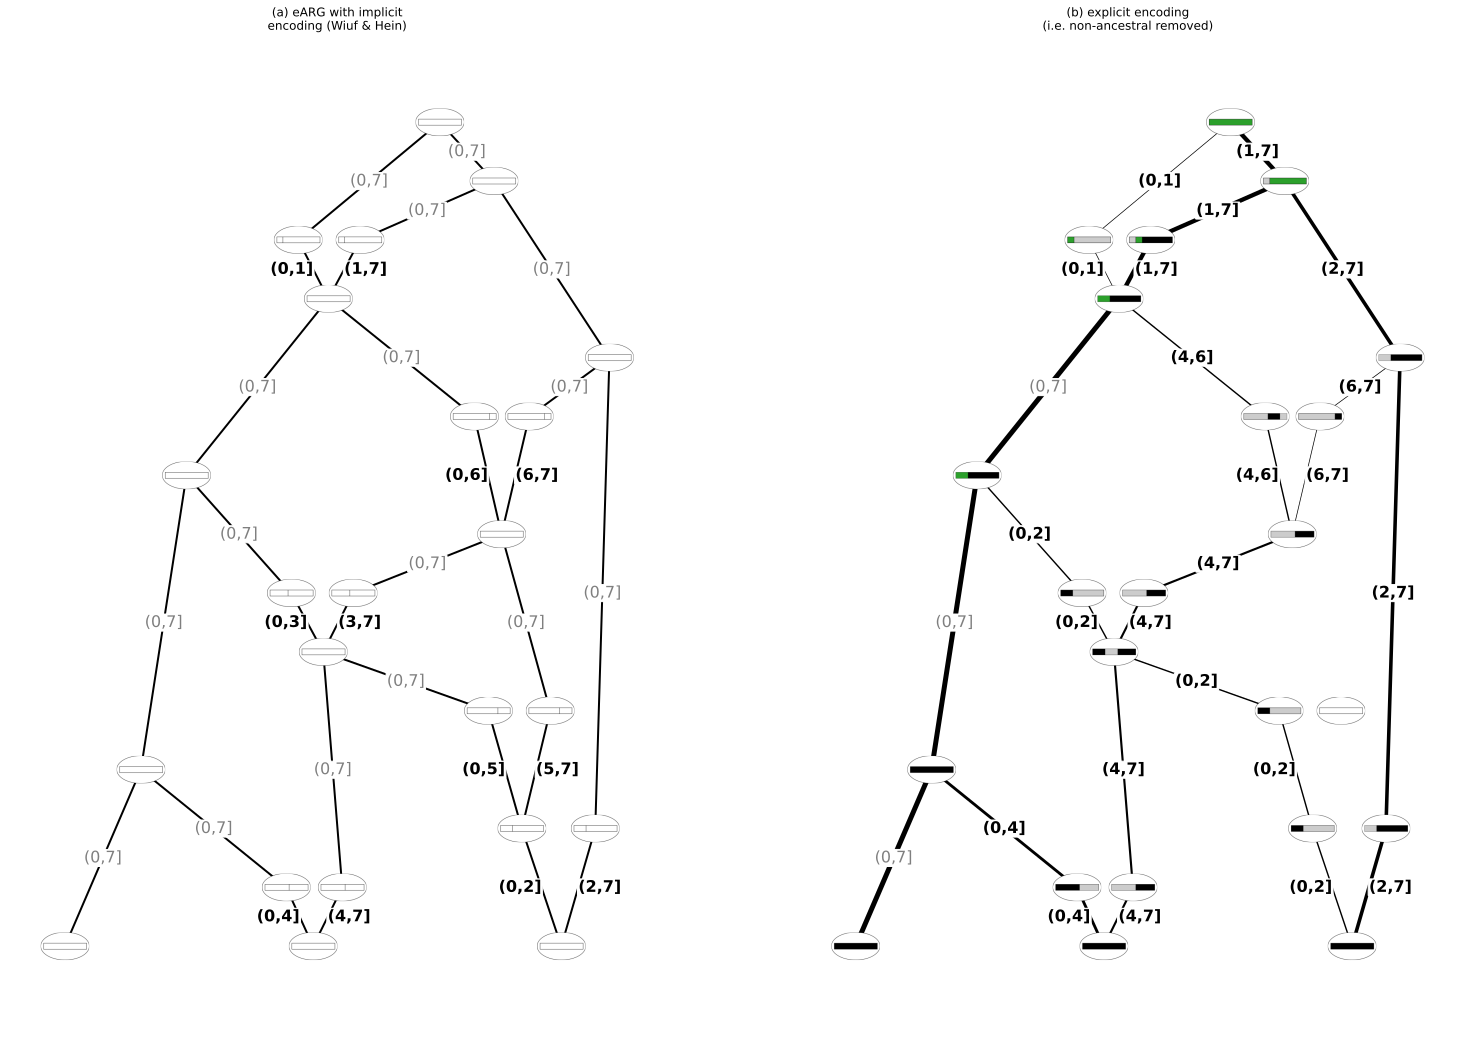
\includegraphics[width=\textwidth]{illustrations/ARG_edge_annotations}
\caption{\label{fig-ancestry-resolution}
Implicit vs explicit edge annotations. (a) An gARG equivalent to the encoding
described by Griffiths can be created by setting all edges to span the full
genome, apart from edges between two recombining nodes and their recombinant
child (edge spans in bold). (b) The sample-resolved gARG, where the Hudson
simplification algorithm has shortened edge spans so that they encapsulate only
the upwards transmission of genetic material from the samples A, B, and C;
plotted line widths are proportional to the genomic span of each edge. The
example ARG used here is taken from \citet[][fig. 1]{wiuf1999recombination}.
}
\end{figure}

Given a GARG $E$ and the set of samples $S$ we can \emph{resolve} its
ancestry by noting that the resolved interval $Ir$ on an edge $(c,p,I)$
is given by [Rough notes]

\begin{itemize}
\item The ``ancestry interval'' $A_u$ of a node $u$ is the union of
all $R_{u, v}$ for all the children $v$ of $u$. (this isn't quite right)
\item The resolved interval is then the intersection of $A_u$ and the
original inheritance interval $I_v$ on the edge.
\item It would be good of if differentiate between the inheritance intervals
 from the GARG and the ancestry intervals of the resolved GARG.
\end{itemize}

This process is illustrated in Fig~\ref{fig-ancestry-resolution}.

\section*{ARG simplification}

Not all nodes in an ARG are equal. Assuming that we have sequenced the
genomes of the samples, there are intrinsic limits on what can
be known about more ancient nodes, determined by the graph topology
and the flow ancestral material through it.
\emph{Simplification}~\citep{kelleher2018efficient} is the process
of removing nodes and re-writing edges in a GARG to remove
various types of redundancy, while maintaining the crucial properties
that the meaningful topology in the local trees is not affected,
and the relationship between nodes in adjacent trees is maintained.

\begin{figure}
\centering
\vspace{5em}
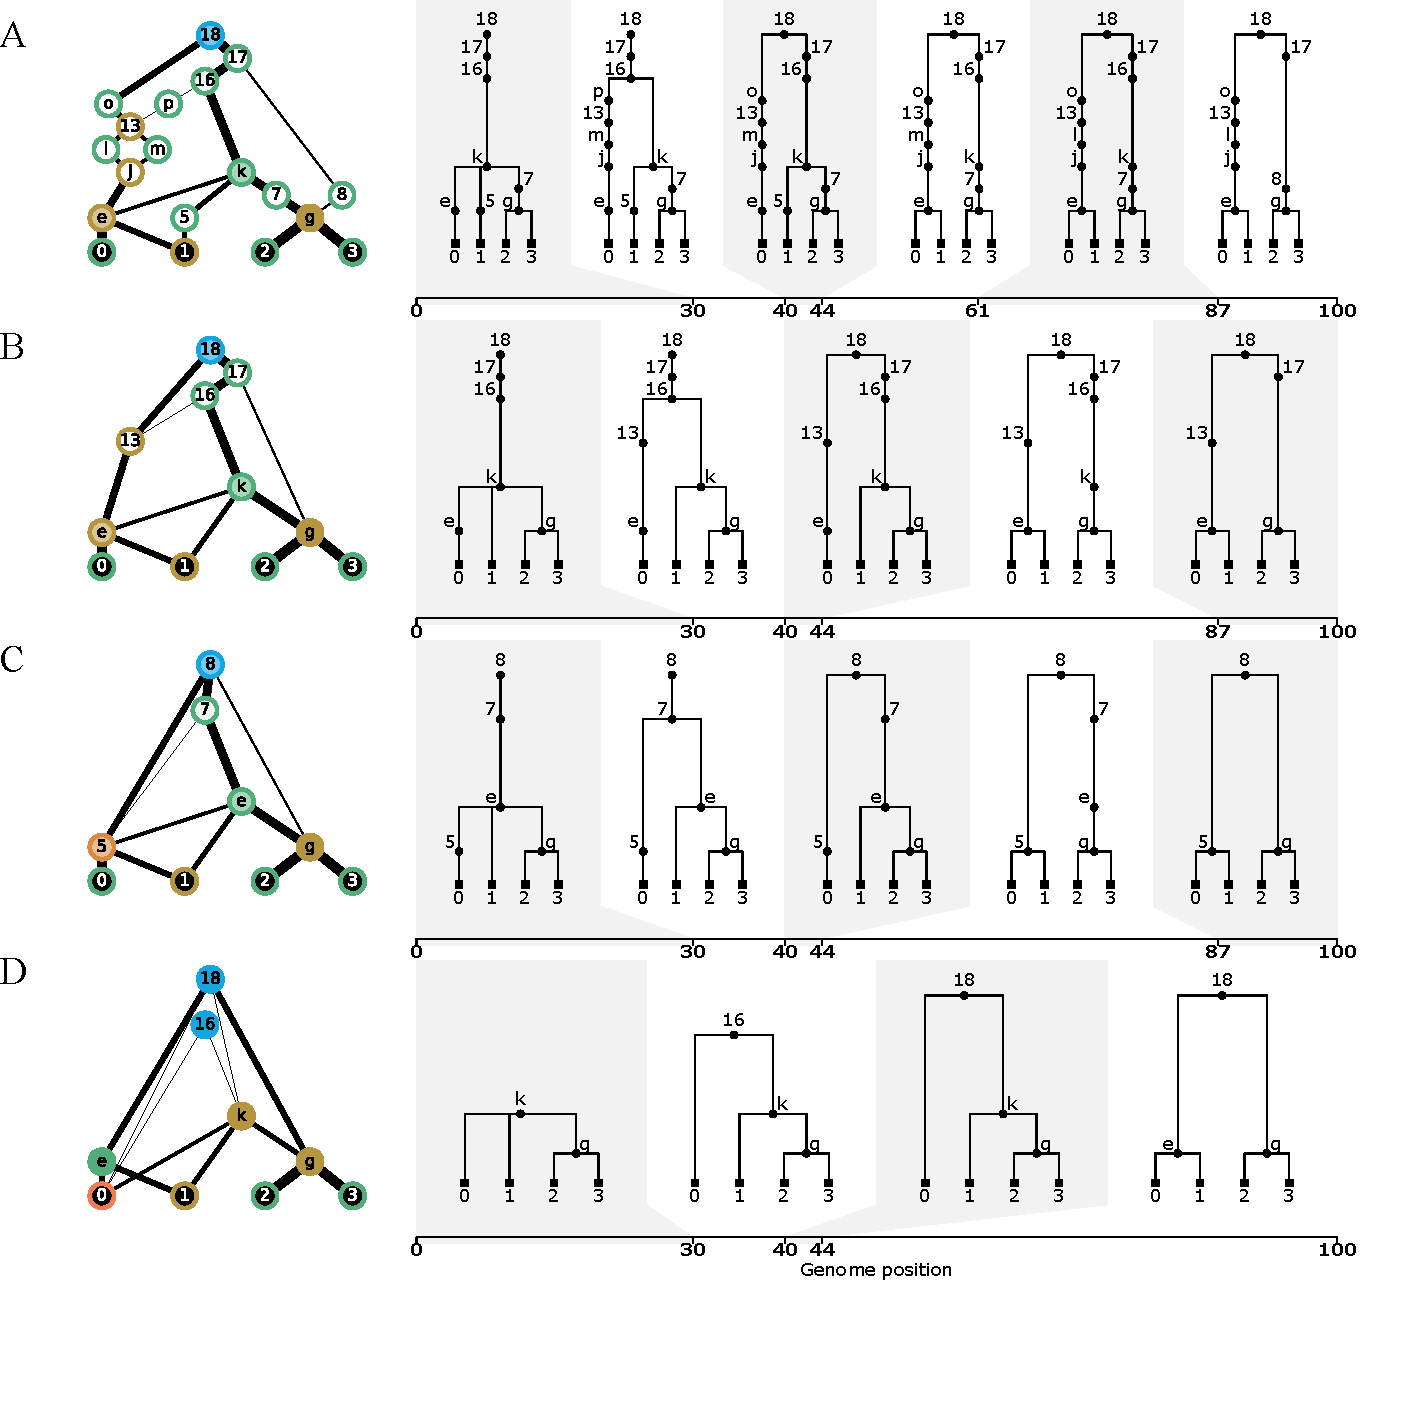
\includegraphics[width=\linewidth]{illustrations/simplification}
\caption{\label{fig-simplification}
ARG simplification. (A) An ARG simulated from a diploid Wright-Fisher
model. Note the complex full-sib relationship between B and C; this
could not be directly represented in a Griffiths-like EARG encoding
(see section XXX).
(B) Simplified to remove all
% trying out this terminology - can define in the text
1-connected graph components (e.g., diamonds).
(C) Remove nodes that are unary in all local trees.
(D) Rewrite edges to skip any unary nodes in local trees.
(E) The local trees for ARG (A).
(F) The local trees for ARG (D).
}
\end{figure}

% Q: would it help to talk about "tree vertices" here or would it
% just be more confusing? I worry that people would think that
% they are two different things then, and it's really important
% that they get that a node-is-a-node
The ideas of ``meaningful'' local tree topologies revolve around the
presence of ``unary'' nodes: a node in the tree that has exactly
one child. For example, Fig.~\ref{fig-simplification}E shows the
local trees along the genome for a simulated ARG
(Fig.~\ref{fig-simplification}A). Consider the right-most tree,
and the path above node $D$. Before $D$ meets its common ancestor
over the interval $(93, 100]$ with the other samples it passes through
nodes $H, K, N, R$ and $S$, reflecting the corresponding
traversal through the ARG (see section XXX). Such unary nodes
in a local tree are not usually considered significant,
because they provide very little information and are not
detectable by information from the tree. % weak
The nodes in a tree usually mark the points where samples find a
\emph{common} ancestor, rather than focusing on specific
ancestors. For most purposes, we would consider an edge
directly joining sample $D$ to the node $T$ to be more
useful and informative. Simplification is the process of removing
these uninformative and (for most computational purposes)
inefficient unary paths.

The first type of simplification that we can perform is to remove
graph topology that is invisible to the samples. The most well
known example of such topology is a so-called
``diamond''~\citep{rasmussen2014genome}
in which the two parent nodes of a recombination immediately
join again into a common ancestor (e.g. $K,N,O$ and $R$ in
Fig.~\ref{fig-simplification}A).
Unless we are specifically
interested in the recombination event or ancestral genomes,
there is no information in this topology and the diamond can b
e replaced by a single edge. More generally, any
subgraph which is singly-connected in both the leafward and
rootward direction (a ``super-diamond'') is non-identifiable and can be
replaced by a single edge. This definition includes the case
of a single node that has one inbound and one outbound edge.
Fig.~\ref{fig-simplification}B shows the result of this type of
graph-level simplification.

Simplifying away diamonds will remove many unary nodes from the
local trees, there can still be nodes that are unary in all
of the local trees. For example, node $H$ is one of the
parents of the recombinant node $D$ is still present in
Fig.~\ref{fig-simplification}B after diamond removal, but
it is unary in all of the local trees since it has an
in-degree of $1$.
Fig.~\ref{fig-simplification}C shows the resulting graph
after removing these nodes.

The remaining nodes are MRCAs of some subset of the samples
at \emph{some} positions along the genome. We still have
some unary nodes in the local trees, but these nodes will
correspond to a coalescence in at least one other
local tree. For example, node $E$ is unary in the first tree
of Fig.~\ref{fig-simplification}E, but is either binary
or ternary in the other trees (recall this is a Wright-Fisher
simulation).

The final level of simplification is to remove \emph{all}
unary nodes from the local trees (Fig.~\ref{fig-simplification}D
and E). [And continue]


% This text might go somewhere
% We may have nodes corresponding to genomes that are ancestral to
% the sample along their entire span
% (e.g.\ node $H$ in Fig.~\ref{fig-ancestry-resolution}),
% genomes that carry no genetic material ancestral to the sample at all
% (e.g.\ node $J$ in Fig.~\ref{fig-ancestry-resolution}),
% and every possibility along the continuum between these extremes.
% Clearly, we can only ever hope to infer the fraction of an ancestor's
% genome that is ancestral to the sample.


\section*{ARG inference methods}
Using the terminology developed here to classify ARGs, we now review methods developed
to explicitly \emph{infer} ARGs from sequencing data.

\subsection*{Parsimony and heuristics}
The problem of reconstructing ARGs for samples of recombining sequences has been of significant
 interest essentially since the ARG was first defined. Early methods focussed on finding the most
 \emph{parsimonious} ARGs, i.e.\ those minimising the number of posited recombination events in
 the history of the sample \citep{hein1990reconstructing}. Two main approaches to explicitly reconstructing
 parsimonious ARGs then emerged: building the ARG either \emph{backwards-in-time} or \emph{along-the-genome}.
 The former approach, introduced by \citet{lyngso2005minimum} and implemented in the program
 \texttt{Beagle}, starts with the input data matrix and reduces it through row and column operations
 corresponding to coalescence, mutation and recombination events, until the empty matrix is reached;
 the corresponding sequence of events can then be used to construct an ARG from the bottom up. The
 latter approach, introduced by \citet{song2003parsimonious} and first implemented in the program
 \texttt{RecMinPath} \citep{song2005constructing}, starts with an initial local tree at some starting
 position, and refines the tree moving left and right along the genome, changing the topology of the
 tree when necessary through \emph{subtree prune and regraft} (SPR) operations (corresponding to
 recombination events).

Reconstructing a most parsimonious ARG for a given data set is NP-hard \citep{wang2001perfect},
and in order to allow for larger input datasets, subsequent parsimony-based methods have resorted
to various relaxations and heuristics. Those utilising variants of the backwards-in-time approach
include the programs \texttt{SHRUB} \citep{song2005efficient}, \texttt{GAMARG} \citep{thao2019hybrid},
and \texttt{KwARG} \citep{ignatieva2021kwarg}, and the method described by \citet{wu2008association}.
Tools constructing genealogies along-the-genome include \texttt{RecPars} \citep{hein1993heuristic},
\texttt{RENT} \citep{wu2011new} and its sequel \texttt{RENT+} \citep{mirzaei2017rent}. Other approaches
include \texttt{TARGet} \citep{camara2016inference}, which implements a method based on topological
data analysis. The scalability of these methods varies substantially based on the heuristics in use
and the underlying data structure, with the most efficient tools limited to analysing hundreds of
sequences.

A number of heuristic methods have also been developed which do not (explicitly) focus on reconstructing
the most parsimonious ARGs, but rather aim for computational efficiency while seeking to achieve good
accuracy of the inferred genealogies. Such methods include \texttt{Margarita} \citep{minichiello2006mapping}
and the approach of \citet{parida2008estimating}; the more recently developed \texttt{Relate}
\citep{speidel2019method} and \texttt{tsinfer} \citep{kelleher2019inferring} use a combination of both
backwards-in-time and along-the-genome approaches, and can be practically used on megabase scale data
and tens to hundreds of thousands of samples under human-like parameters.
Another class of methods has recently emerged that use a \emph{threading} approach, constructing ARGs
by adding sequences to the graph one-by-one. Originally introduced by \citet{rasmussen2014genome} as a
way of generating MCMC proposals for ARGs, a similar idea was leveraged in \texttt{ARGneedle}
\citep{zhang2021biobank} to reconstruct ARGs for biobank-scale data.
% AI: just to note, these papers do not all agree in their definition of an ARG.
% I guess this is one of the points of the present paper, but should we mention this fact?
% Should we also mention that most of these infer just the topology, but some also the times?

\subsection*{Model-based methods}
An alternative approach is to treat the ancestry as a latent parameter to be averaged out
by Monte Carlo methods, based either on importance sampling
\citep{griffiths1996ancestral, fearnhead2001estimating, jenkins2011inference}
or MCMC \citep{kuhner2000maximum, nielsen2000estimation, wang2008bayesian, fallon2013acg}.
These methods invariably operated on a representation of the ``little ARG'', typically
generated until the grand MRCA. They are extremely computationally expensive,
and applicable to at most hundreds of samples consisting of tens of kilobases with
human-like parameters.

Due to the computational expense of sampling ``little ARGs", state-of-the-art
Monte Carlo methods typically rely on cheaper, approximate models.
The most prominent examples are \texttt{ARGWeaver} \citep{rasmussen2014genome}
and \texttt{Arbores} \citep{heine2018bridging}. The former also utilises a time
discretisation approximation, but scales to dozens of mammal-like genomes.
The \texttt{ClonalOrigin} method \citep{didelot2010inference,
medina2020speeding} uses the \texttt{ClonalFrame}
model and data structure, though it is not as scalable as \texttt{ARGWeaver}.

A very recent MCMC method called \texttt{ARGInfer} has resulted in the first
improvement in the scalability of Monte Carlo methods for the exact ARG model
by making use of the tree sequence representation of marginal trees, suitably enriched
to facilitate the computations needed for MCMC sampling \citep{mahmoudi2021inference}.
While not competitive with the scalability of \texttt{ARGWeaver}, \texttt{ARGInfer} extends
the feasible range of sequence lengths by at least an order of magnitude when
compared with methods which sample realisations of the exact ``little ARG''.


\begin{figure}
\vspace{5em}
\caption{\label{fig-inferred-args}
ARGs inferred by different methods from a small dataset. Notes about these
ARGs.
}
\end{figure}

\section*{Discussion}

Discussion points (may or may not be used, certainly would be heavily revised)

\begin{itemize}
\item It is unfortunate that we are adding yet another meaning to the
term ARG here, but all we're really doing is making the implicit
assumptions that others have made (i.e., describing the output of
Relate, tsinfer etc as ARGs) and making them concrete. We need to have a
term to describe all of these things, and since people are already using
ARG for this, we might as well make it rigorous. We can then move away
from the unfruitful discussion about which methods infer a ``true'' or
``real'' ARG (none do, really, under the original definitions) and
instead start discussing the \emph{properties} of these ARGs. (See
next point also.)
\item Terminology based around an inferred ancestry being a ``true''
ARG is impoverished and misleading. The only reasonable interpretation
of a ARG being true or not is whether it's a sample from the coalescent.
Most inference methods (and all that scale well) do not. In any case,
the coalescent is just one model, and a highly idealised one. It is
exceedingly unlikely that the actual ARG describing the ancestry
of any biological population is ``true'' ARG in this sense. The terminology is
impoverished because it reduces the possibilities available
to something either being an ARG or not, whereas there are many different
interesting properties of these structures that we should be able to
discuss and compare.
\item tskit can represent any ARG.
\item Interchange is a real problem, and if we're going to realise the
potential for ARGs in genomics we must solve it. Efforts to standardise
phylogenetic networks haven't done very well (~\citep{cardona2008extended}
has 89 citations). The only real effort to standardise an ARG format
based on extending GraphML~\citep{mcgill2013graphml} has 11 citations.
GraphML~\citep{mcgill2013graphml} has some of the same key ideas
as tskit though, in particular allowing the annotation of ``live sites''
to an edge as a set of disjoint intervals that hold ancestral material.

\item There are real computational disadvantages to the Griffiths ARG
data structure. Having two types of node (three really, as we need
``sample'' nodes which are also treated differently) complicates algorithms,
and makes it difficult to reason about the structure of the ARG as a
graph. For example, there's some weirdness about mutations over
recombination nodes discussed by Gusfield [Ana?]

\item Comparison metrics are a problem. All evaluations has essentially
looked at either some form of pairwise comparison of trees along the genome
using tree metrics, or looked at the distributions of TMRCAs. No
one has succeeded in performing any comparisons of ARGs beyond
regarding them as a sequence of independent trees. If we genuinely believe
that ARGs are more than this, then we need to devise some metrics that
consider more than the local tree structure.

\item We should discuss other types of ancestry network also.
The crucial distiction between an ARG and a phylogenetic network (I think?) is
the presence of position information specifying the location of
recombination events (and by extension, the complete passage
of ancestral material the graph). Without position information
we know that a particular node was an ancestor somewhere along the
sequence, but not exactly where.

\item We make the point about expressivity of the EARG pretty
hard, but we don't mention anything about indels and structural
rearrangements etc. It's probably worth mentioning genome graphs
somewhere just to fend off this criticism. The high-level point
would be that it's unlikely to be easier to model this stuff
using node annotations.

\end{itemize}

% TODO not clear this belongs in the discussion, but we'll definitely
% want to make some of these points, even if they are being repeated
% from earlier section.
It is difficult to imagine a practical calculation performed on an
ARG that does not involve either the sequential generation of trees
along the genome or the resolved ancestry segments.
Knowing the resolved segments in an ancestry resolved GARG allows
us to perform many calculations without explicitly generating
the trees, and lets us work with the ancestry on a genome-by-genome
basis. We give three examples here. Firstly, generating mutations
on edges can be performed very quickly on an ancestry resolved
GARG, since we only need to examine $O(|E|)$ edges rather than
$O(nt)$ tree branches (assuming $n$ samples and $t$ marginal trees)
~\citep{baumdicker2021efficient}. If the ancestry were not resolved,
we would generate a large number of mutations on areas of the edge that
are non-ancestral. Secondly, computing the likelihood of a given
ARG realisation under the coalescent with recombination model
requires that we essentially recapitulate the state of Hudson's
algorithm (see XXX section) at each node in
the graph~\citep{baumdicker2021efficient}. Having resolved ancestry
substantially simplifies this process. Thirdly, computing
[FIXME describe what we did in tsdate]~\citep{wohns2021unified}.

Sequentially generating the marginal trees along the genome
is also fundamental, and is necessary whenever we need to
perform calculations that are contingent on more than just the
isolated properties of an edge. \cite{kelleher2016efficient}
showed how all trees can be sequentially generated in
constant time per tree transition in a fully simplified GARG.
Furthermore, we can easily reason about how tree topologies
change (and stay the same), leading to efficient algorithms
for computing population genetic
statistics~\citep{kelleher2016efficient,kelleher2018efficient},
implementing the Li and Stephens
model~\citep{kelleher2019inferring,wohns2021unified}
and likely many more.



\bibliographystyle{plainnat}
\bibliography{paper}

\end{document}
